\chapter{Implementation}

% Section Introduction


\section{Type System}
The type system for the DSL is built using a subset of Scala, Python, and Cassandra's type systems. These types are shown in Figure \ref{fig:datatypes}.

\begin{figure}[h]
	\centering
	\begin{tabular}{| c | c | c | c |}
		\hline
		\textbf{Base Type} & \textbf{Python} & \textbf{Scala} & \textbf{Cassandra} \\ \hline
		Integer & int & Long & bigint \\ \hline
		Float & float & Double & double \\ \hline
		String & string & String & text \\ \hline
		Boolean & boolean & Boolean & boolean \\ \hline
		DateTime & datetime & Instant & timestamp \\ \hline
	\end{tabular}
	\caption{Primitive Types}
	\label{fig:datatypes}
\end{figure}

There were two main goals when selecting these primitive types. Firstly, every type should be able to be represented without data loss in all parts of the system. Secondly, it should be possible to represent the types in protobuf format, as this would allow for easy serialisation of result data. All types except DateTime are can be converted to protobuf natively, and DateTimes are supported by serialising as an ISO8601 formatted string \cite{iso_8601}.

Designing the actual interfaces to represent these values presents a challenge. To be able to read and manipulate these types in Scala at runtime, the raw primitive types cannot be used. This is because the only common supertype of all primitive types is \textit{Any}, as shown in Figure \ref{fig:scala-unified-types}. There is effectively no information shared between all supported types in the system. To discover which type a given value is (or if the type is even supported), the system would have to perform runtime type checks against all possible supported types. These checks would add a significant amount of overhead, and as a result this approach was not selected.

\begin{figure}[h]
	\centering
	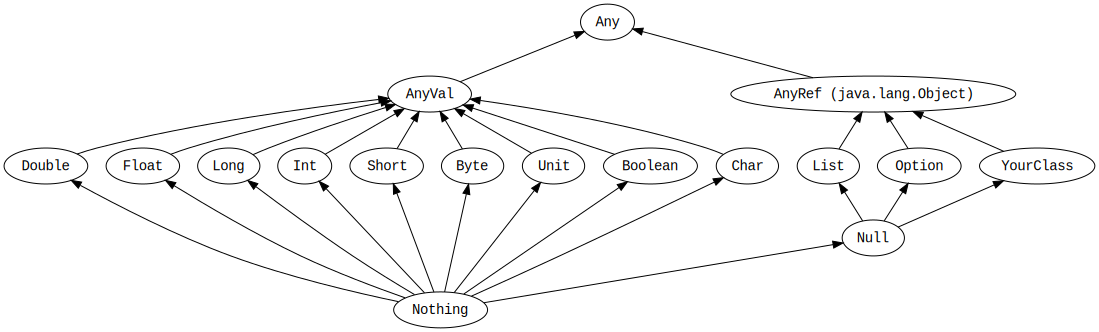
\includegraphics[width=0.8\textwidth]{chapters/diagrams/implementation/unified-types-diagram}
	\caption{Scala Unified Types \protect\cite{scala_unified_types}}
	\label{fig:scala-unified-types}
\end{figure}

Another possible approach to solving this problem is to create a lightweight container class, which holds the value, and the type information about the value at runtime. This means that the system only needs to perform the runtime type check once in order to create the correct class instance. Due to limitations of Java, this conceptual solution is not entirely straightforward to implement. The container class would use a generic type parameter which stores the type information of the value inside the container. A given row of data would need to support multiple types of data stored together, and this is not possible using generics as the type information of the generic is erased at runtime \todo{reference}. 

The container class could instead be defined as an interface, and each supported type provides an implementation of that interface, but this is not much better than the primitive type solution, as the runtime type check simply becomes a runtime pattern match on the class instance. A solution that exploits some kind of polymorphism is preferred.

Scala provides an feature known as ClassTags \todo{reference}. These allow the erased type information to be recorded, and also allow equality checks to be performed between ClassTags. By storing a ClassTag instance, we can implement type equality checks between values in the system, to determine if they are of the same type. Furthermore, we can use this type information later to determine what types are accepted and returned by FieldExpressions.

This is defined in the system using a base interface \textit{ValueType}, which captures the ClassTag requirement. This interface is used as part of both \textit{TableField}, which captures field information (name and type), and \textit{TableValue}, which captures value information (value and type). Implementations for all the supported types are then provided for both \textit{TableField} and \textit{TableValue}. \todo{insert figure ref} shows the hierarchy of these types. 

\missingfigure{ValueType - TableField - TableValue hierarchy} 

\subsection{Result Model}
This hierarchy of classes provides everything needed to define computation results in the system. Headers are defined as a sequence of TableFields, and results are defined as a two-dimensional array of \texttt{Option[TableValue]}. As defined in the requirements, null values must be supported, but the use of nulls in Scala is discouraged. Instead, Option is preferred as it is supported by all the typical functional methods. In this model, values are represented by \texttt{Some(TableValue())}, and null values are represented by \texttt{Nothing}. \todo{insert figure ref} shows what an example result looks like using this definition.

\missingfigure{Visual of TableResult}

\section{Domain Specific Language}
The user's interaction with the framework is driven entirely by the Domain Specific Language (DSL). The language allows the user to define expressions, comparisons, aggregates, and then use these to define computations like Select, Filter and Group By. As per the requirements, the DSL has been modelled with SQL-like syntax.

\subsection{FieldExpressions}
FieldExpressions are the key building block of the DSL. They allow the user to define arbitrary row-level calculations to be used as part of more complex operations. FieldExpressions are defined as an interface, which provides a standard set of methods, and there are three subclasses that provide implementations:

\begin{itemize}
	\item Values: define literal values which never change across all rows
	\item Fields: when iterating over the rows of a result, gets the value from the named field in the current row.
	\item FunctionCalls: perform arbitrary function calls using further FieldExpressions as arguments.
\end{itemize}

Examples of FieldExpressions are shown in Figure \ref{fig:field-expressions-examples}.

\begin{figure}[h]
	\centering
	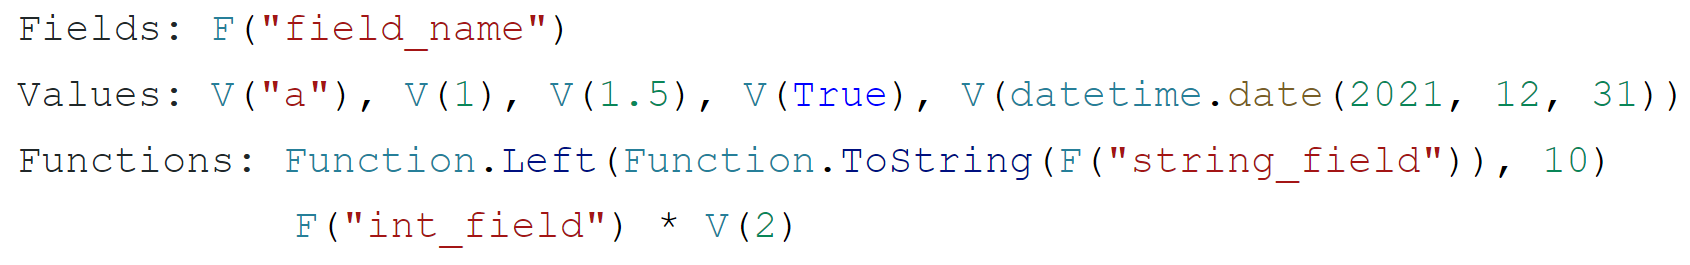
\includegraphics[width=0.8\textwidth]{chapters/diagrams/implementation/field-expressions-examples}
	\caption{Examples of FieldExpressions}
	\label{fig:field-expressions-examples}
\end{figure}

Many basic functions have been implemented, including arithmetic, string and cast operations. However, the function system is designed to be extensible. A number of helper classes are defined to allow the creation of basic unary, binary and ternary functions, but FunctionCall is itself an interface which can be given completely custom implementations if required. The main constraints on the functions that can be defined are that only the 5 primitive input types are supported.

\paragraph{Type Resolution} 
Type Resolution on FieldExpressions is performed in two stages: a resolution step, and an evaluation step. The resolution step takes in type information from the header of the input result, and verifies that the FieldExpression is well typed with regards to that result. This is necessary for Fields, which may be valid for one result but invalid for another, for example if the field name is missing from the result. The evaluation step performs the computation on a row from that result without any type checking. 

This two-step process has a number of benefits. The resolution step enables a form of polymorphism on some functions like arithmetic operations. At the resolution step, these functions determine what types are returned by their sub-expressions, and resolve to the correct version for evaluation. For example, the add function can resolve to AddInt, AddDouble, or Concat for strings. Also, there is reduced overhead at runtime as type checking does not need to be performed for each row - unchecked casts are used here instead.

\paragraph{Named Expressions}
When performing a Select operation, the output fields are all expected to be named. This allows the user to repeatedly chain operations by referencing fields from the input. Therefore, FieldExpressions have a method to allow them to be named. When this method is called, the FieldExpression is wrapped as a tuple with the name into a NamedFieldExpression. Field references are able to reuse their previous name automatically to reduce the need for repeated naming calls. 

% Abstract class implementation
% - isWellTyped
% - doesReturnType
% - resolve/evaluate steps
% - named/unnamed

\subsection{FieldComparisons}
FieldComparisons are another key building block of the DSL. They allow the user to define arbitrary row-level comparisons. FieldComparisons use a two-step resolution-evaluation process. This is in place to accommodate the two-step process that already exists for FieldExpressions. They are defined as an interface, and there are four subclasses that provide implementations:

\begin{itemize}
	\item Null Checks: takes a single FieldExpression as input, and filters out rows where it is null/not null.
	\item Equality Checks: performs an equal/not equal check on two FieldExpressions.
	\item Ordering Checks: applies an ordering comparator to two FieldExpressions.
	\begin{itemize}
		\item Supports $<$, $<=$, $>$, $>=$.
	\end{itemize}
	\item String Checks: applies a string comparator to two FieldExpressions
	\begin{itemize}
		\item Supports contains, starts with and ends with (both case sensitive and insensitive versions).
	\end{itemize}
\end{itemize}

Examples of FieldComparisons are shown in Figure \ref{fig:field-comparisons-examples}.

\begin{figure}[h]
	\centering
	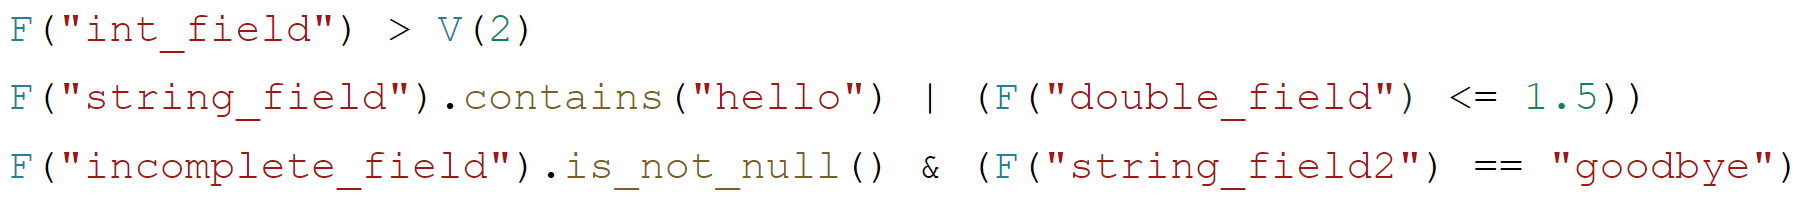
\includegraphics[width=0.8\textwidth]{chapters/diagrams/implementation/field-comparisons-examples}
	\caption{Examples of FieldComparisons}
	\label{fig:field-comparisons-examples}
\end{figure}

\paragraph{Combined Comparisons}
The user is able to combine multiple FieldComparisons using AND/OR operators. This is a lightweight wrapper around Scala's own AND (\texttt{\&\&}) and OR (\texttt{||}) boolean operators, meaning optimisations like short circuiting operate as normal with no extra work.

\subsection{Aggregate Expressions}
Aggregate Expressions are the final part of the DSL. These are used only as part of Group Bys, and allow the user to define methods of aggregating all rows of a result. Aggregate Expressions take a NamedFieldExpression as an argument, and compute a single row output from any number of input result rows.

The system supports Min, Max, Sum, Average, Count, and String Concatenation operations. These aggregates are polymorphic where possible. For example, minimum and maximum handle numeric types numerically and strings lexicographically.

\todo{expand + examples}

\subsection{Protocol Buffer Serialisation}
All components of the DSL have been designed to be serialised to protobuf format. This allows any queries written by the user to be passed around the system using gRPC, and if required the query can also be serialised to a file. The results of a query are also serialisable, to allow the system to return query results to the user. gRPC has a size limit of 4MB for individual messages, so results are split up by row and streamed individually.

\subsection{Python Implementation}
The Python frontend is designed to be straightforward to use, hiding the complexities of the computation being performed in the backend. A number of Python-specific features were used to help with this.

Python allows developers to override common operators, including arithmetic ($+$, $-$, $*$, $/$) and comparison ($<$, $>$) with custom definitions. These are known as double underscore \textit{(dunder)} methods. The Python implementation of FieldExpression overrides the arithmetic operators, as well as comparison operators to allow the user to automatically generate function calls and FieldComparisons, without having to write the full, verbose definition.

Furthermore, query results can be converted from their protobuf definition as received from the server to a pandas DataFrame \cite{reback2020pandas}. This decision was made because pandas is one of the most commonly used frameworks for data analysis in Python. In the 2022 Stack Overflow Developer Survey, it was the third most popular non-web framework \cite{stackoverflowsurvey2022}. Therefore, it is likely that the intended users of the system will have prior experience performing data processing using DataFrames.


\section{Minimum Viable Product}
To break development into more manageable chunks, a minimum viable product (MVP) was implemented first. This required implementing partitioning of Cassandra Source Data, and the Select and Filter operations. By taking this approach, any issues in the design of the system could be discovered and rectified earlier. Also, this would ensure that modules built for the MVP were reusable, as they would be designed with the purpose of integrating into the full solution.

Group By partitioning would not be implemented for the MVP, meaning all operations available to the user are row-level, and only one set of partitions need to be generated for a query. This removes the need for state in the workers, greatly simplifying their design at this stage.

The below diagrams are provided to give a high-level picture of how the MVP system operates. The Orchestrator manages calculating partitions, delegating them to workers, and collating final results. 

\todo{insert figure here} shows the data flow for the Orchestrator.

\missingfigure{MVP Orchestrator Flow}
% Calculate partitions from Cassandra
% Delegate partitions to workers
% Compile results and return to user

\todo{insert figure here} shows the data flow for all Workers.

\missingfigure{MVP Orchestrator Flow}
% Accept a single partition for a query from Orchestrator
% Fetch partition data from Cassandra
% Compute result
% Return result to Orchestrator

\subsection{Cassandra Partitioning}
The goal of the partitioning module is to split up the source data into roughly equal chunks of a manageable size. As described in the Design Chapter, Cassandra was selected as the persistent storage module because its storage model closely matches the type of partitioning the system requires. 

When data is stored in Cassandra, the primary key of each row already has a 64-bit token assigned to it. Cassandra allows queries to filter on ranges of these tokens, meaning the data can be split up and read from the database in chunks. To be able to ensure the partitions are a manageable, defined size, an estimate of the size of the full source data is required. Cassandra provides this information in the \texttt{system.size\char`_estimates} table. This table provides an estimate of the size of each table in the database, and these are generated automatically every 5 minutes \todo{Reference}.

From a size estimate of the full table, estimates can be calculated for any given token range using the equation in Figure \ref{fig:token-range-estimation}. The fraction calculates the percentage of all tokens that the given token range represents.

\begin{figure}[h]
	\centering
	\[ \frac{\text{Number of Tokens in Token Range}}{\text{Total Number of Tokens: } ((2^{64}-1) - (-2^{64}))} \times \text{Estimated Table Size} \]
	\caption{Token Range Size Estimation Equation}
	\label{fig:token-range-estimation}
\end{figure}

It is the orchestrator's responsibility to generate an allocate the partitions to each worker. Using this equation, it first gathers the token ranges which each node is responsible for storing. Then, it performs a joining and splitting process over each node, depending on the size of the token ranges. The flowchart in Figure \todo{insert missing figure} shows the full process for generating the output partitions.

% Example split and join
% After split/join, each partition, which contains one or more token ranges should be roughly equal to the chunk size, which is set in settings.

\missingfigure{Flow diagram of partitioning process}
% Get size estimates of table
% Get token range ownership for each node
% Iterate over all nodes
% iterate over all token ranges for this node. Is size of token range larger than partition size?
% - Yes - split
% Iterate over all token ranges for this node. Is size of this token ranges in node less than partition size? 
% - Yes - combine with next token range
% - No, this becomes a partition, move to next token range
% Output - partitions for each node

Figure \todo{insert missing figure} demonstrates how the splitting process works. The system calculates how much times larger the token range currently is than the goal partition size, then splits the 

\missingfigure{splitting process - equation and example}

Figure \todo{insert missing figure} demonstrates how the joining process works. Given a sorted list of token ranges, the system repeatedly adds sequential elements to a partition until it is larger than the goal partition size. Then, the partition is marked as completed. The list is sorted by size ascending to ensure the smallest number of partitions are created - if there are a large number of very small token ranges, these will be combined into a single large partition together.

\missingfigure{joining process - equation and example}

The Cassandra Java Driver provides a wide range of helper functions for performing the joining and splitting of token ranges accurately to produce new token ranges. The system simply calculates how much joining or splitting is required based on the size of the token ranges and the table size estimate. It then uses the driver to perform the calculations.

\subsection{Cassandra Data Co-Location}\label{subsec:colocation}
Once the list of partitions for each Cassandra node are generated, the system attempts to co-locate workers to Cassandra nodes. The goal of this process is to produce an \textit{optimal assignment} of partitions, where each partition is matched to one or more workers to minimise network latency when fetching the data from Cassandra.

To do this, each worker first calculates its closest Cassandra node. This is done by opening a TCP connection multiple times with each Cassandra node, and averaging the time taken over multiple attempts. The node with the lowest average latency is selected as the closest node. Figure \todo{insert figure here} shows this process.

\missingfigure{worker latency calculation diagram}

The orchestrator uses this information to match each worker to a Cassandra node and its corresponding list of partitions. The output is an optimal assignment between workers and partitions. It's possible for more than one worker to be matched to the same set of partition, and it's also possible for a set of partitions to have no co-located worker nodes. In this case, they are kept as unassigned, and the work assignment algorithm handles their allocation. Figure \todo{insert figure here} shows an example optimal assignment after this process is complete.

\missingfigure{worker optimal assignment to partitions diagram}

\subsection{Work Assignment}
Given an optimal assignment between workers and partitions, the orchestrator manages the process of sending requests to all workers to compute the partitions. A simple solution to this problem would be to iterate through the optimal assignments in order for each worker, delegating work when a request finishes and stopping when the list is empty. However, this can result in idle workers, for example if one worker's list of optimal assignments is shorter than the others, or if one worker takes unexpectedly long to complete their work.

The ideal solution would ensure a worker first computes all of its own optimal partitions and, once these are complete, computes the partitions that were originally assigned to other workers. This implements a form of dynamic load balancing, because a faster-running worker is able to take on more requests than a slower worker, and no worker will be idle unless there are no partitions left to be computed.

However, this presents concurrency challenges, including preventing race conditions like the same partition being delegated twice to different workers. The final approach taken to solve this uses the actor model, first introduced in 1973 by Carl Hewitt \cite{hewitt1973session}. Specifically, the Akka Actors framework was chosen, as it is one of the most widely supported implementations of this model for Scala \todo{reference docs}. The actor model abstracts away the complexity of synchronisation and thread management. Instead, components of the system become actors. Each actor defines a set of messages that it accepts, and the response to each message. The framework provides a guarantee that an actor will only ever process one message at a time.

The solution models the optimal partitions as \textit{producer} actors, and the workers as \textit{consumers}. Producers will respond to requests for work with partitions, and will shut down when all partitions have been given out. Consumers are provided with an ordered list of producers, then repeatedly request and compute work from each in order. When all assigned producers for a consumer are empty, the consumer will shut down. Each consumer is given a list with a different order, with the producer of that consumer's optimal partitions placed first in the list. 

This solution also handles the case where no worker is co-located with a set of partitions, as this producer will simply be placed at the end of the list of producers for each consumer. As a result, these partitions will eventually be processed.

% Include this? possibly confusing
The final part of this solution is an \textit{assembler}, which compiles the results from each consumer into a complete result. When all results are received, the assembler sends the result data back to the user.

Figure \todo{insert figure here} provides a visual representation of the model.

\missingfigure{Producer Consumer Model}

\subsection{Result Computation}
Once partitions have been delegated to the workers, performing the computation is relatively straightforward. Included below are descriptions of how the Select and Filter operations are performed.

\paragraph{Select} 
This operation takes any number of NamedFieldExpressions. To compute a result, apply each NamedFieldExpression to each row of the input result. The output result has the same number of rows as the input, and fields equal to the number of NamedFieldExpressions. 

Figure \todo{insert figure here} shows how a Select is computed.

\missingfigure{Select Computation}

\paragraph{Filter}
This operation takes a single FieldComparison, or a number of FieldComparisons combined using boolean operators. To compute, apply the comparison to each row of the input result, removing any rows where the comparison returns \texttt{false}.

Figure \todo{insert figure here} shows how a Filter is computed.

\missingfigure{Filter Computation}

Selects and Filters can be applied repeatedly, in any order from the source dataset to design a query. Figure \todo{insert figure here} shows an example query calculation using a series of Select and Filter operations. This process is repeated for each partition.

\missingfigure{Calculation of Source -> Select -> Filter -> Output}
	
\section{Overall Solution}
The main change from the MVP to the final solution is to add Group By operations. However, this is the first operation that cannot be computed row-by-row, which introduces a significant amount of complexity, as the worker nodes will now need to be stateful. In particular, the workers will have to cache partial results, and communicate with one another to generate new partitions for the Group By operation. This change also introduces further complexity for the Orchestrator, as it will have to manage the states of each worker, and ensure the worker state is cleared after a query completes.

% Overview of final model
% Diagram of orchestrator and worker model - incoming and outgoing requests
% Orchestrator - collate results from workers
% Worker - same as before, but stateful

\subsection{Data Model}\label{subsec:data-model}
% This section should be clear and understandable, as much of the rest refers to partial and full versions
The data model is split into two key components: \textit{DataSource} and \textit{Table}. DataSource is an interface, representing any part of the query where new partitioning is required to continue, including Cassandra Source Data, and Group By operations. Table is a class, representing any part of the query that contains purely row-level computations, including Select and Filter operations. Tables depend on a specific DataSource. 

Optionally, DataSources can have dependent Tables which must be calculated first. For example, a Group By DataSource requires a single Table to be fully computed before it can be generated. A Cassandra DataSource will always act as the terminal component for a query, as it has no dependencies. 

Furthermore, DataSources and Tables also have a partial form, which represents part of the full source dataset. \textit{PartialDataSource} is also provided as an interface, as the implementation is different depending on how the dataset is partitioned. \textit{PartialTable}, is essentially a duplicate of Table, but references a PartialDataSource rather than a DataSource.

Any query the user writes is made up of a mix of DataSource and Table components. Figure \todo{insert figure here} shows the outline for a Filter and Select query. 

\missingfigure{Filter/Select query datasource table}

Figure \todo{insert figure here} shows the outline for a more complex query including a Group By. Note that any number of Select and Filter operations can be placed in the Table component, as no new partitions are required to produce the result.

\missingfigure{Group By Query}

\subsection{Data Store}
The data store is a core worker component in the overall solution. It allows the workers to store partially computed data, which can be referenced again in later parts of the query execution. In particular when workers are communicating with one another, it is likely that the worker will be processing more than one request at the same time. Therefore, Akka Actors is used again in this component to simplify the implementation of the data store, by ensuring it only processes one request at a time.

The data store is modelled as an actor which contains three kinds of data: results, partitions and hashes. Results contain a set of outputs for a Table computation, partitions contain a set of outputs for a DataSource computation, and hashes are used in the process of computing a Group By partition.

The data store provides a set of create, read, and delete operations for each of these types of data, as well as helper functions for managing the data store state. Figure \todo{insert figure here} shows the architecture of the data store. 

\missingfigure{Table store architecture diagram}

The data store is designed using two lookups at each stage. First, the full version of the data is looked up, then the partial version. Partial forms of Tables and DataSources always contain a reference to the full version, but not the other way around. Therefore, this decision does not increase the time taken to insert new data significantly, but it does improve the speed of get and deletes, which would otherwise require searching the entire data store to find the items to get or delete.

\subsection{Query Plan}
By separating Tables and DataSources, a generic framework for executing queries can be designed. This is known as a Query Plan. The Orchestrator is responsible for generating and managing the execution of query plans when the user makes a request. 

A Query Plan is made up of a sequence of \textit{QueryPlanItems}, which is an interface defining some part of a query plan. Each QueryPlanItem has an \textit{execute} method, which will make some change to the state of all workers in the cluster when called. There are four main QueryPlanItems, which allow DataSources and Tables to be calculated and deleted, and both DataSource and Table have a function that generates the full Query Plan to compute their output from scratch.

Figure \todo{insert figures here} shows the query plan generated for the Filter and Select query and the Group By Query shown in \ref{subsec:data-model}.

\missingfigure{Select and Group By query plan}

\paragraph{GetPartition}
This is the most complex QueryPlanItem, encapsulating a number of steps in order to compute and store the partitions of a DataSource. There are two main flows depending on if the DataSource has dependent Tables.

If the DataSource has no dependencies, for example when pulling data from Cassandra, then Figure \todo{insert figure here} shows the process for this item. 

\missingfigure{Flow with no dependencies}

If the DataSource has dependencies, for example when computing a Group By operation, then Figure \todo{insert figure here} shows the process for this item. The details of the hashing process are abstracted behind the \textit{DataSource} interface from the perspective of GetPartition, but further details of how this is implemented for Group By can be found in \ref{subsec:group-by}.

\missingfigure{Flow with dependencies}

In both cases, GetPartition needs to manage the process of sending the requests to the workers to actually compute the partitions.
% Integrate earlier actor system code here

\paragraph{PrepareResult}
The aim of this QueryPlanItem is to compute a Table from partitions of a DataSource that are already stored on the workers. Therefore, it will always be called after GetPartition, with the partitions generated by GetPartition as an argument. It uses a modified version of GetPartition's actor system to iterate through all partitions stored on each worker, sending a request for each to perform the Table computation for that partition.

\paragraph{DeleteResult and DeletePartition}
There are also delete operations to remove a result when it is no longer required, \textit{DeletePartition} and \textit{DeleteResult}. These will send a single request to each worker to delete a specific Table or DataSource. The workers will remove all results that relate to that Table or DataSource, and respond with a confirmation.

\subsection{Group By}\label{subsec:group-by}
The Group By operation takes any number of NamedFieldExpressions to act as unique keys, as well as any number of aggregate expressions which will be computed for each combination of unique keys. As with pulling source data from Cassandra, the goal when computing a Group By is for the partitions generated to be roughly equal chunks of a manageable size. As before, to do this, two things are needed: an estimate of the full size of the dataset, and a way of splitting the dataset up to keep unique keys together.

The four-step process of calculating hashes, shuffling data, computing the result and deleting the original hashes is all controlled by the query plan execution in the orchestrator

\paragraph{Hashing} To estimate the size of the full dataset, an existing class, \textit{SizeEstimator}, from Apache Spark was used, with a small number of changes for compatibility with Scala 3 \todo{reference}. This class provides a static method \textit{estimate} which accepts any Scala object and produces an estimate, in bytes, of the size of the object. This can be called on all partial results across all workers, and the results totalled to calculate the total size of all data for a Table. Figure \ref{fig:group-by-num-partitions} shows how the size estimate can be used to derive the total number of partitions to generate for a Table.

\begin{figure}[h]
	\centering
	\[ \frac{\text{Table Size Estimate}}{\text{Goal Partition Size}} \]
	\caption{Group By - Total Partitions}
	\label{fig:group-by-num-partitions}
\end{figure}

Hashing, combined with the modulo operation, is used to determine which partition each row should be assigned to. In particular, Murmur3Hash is used as the hashing algorithm, which is the same as in Cassandra and is provided natively by Scala. Figure \ref{fig:group-by-partition-assign} shows the high level equation for assigning rows to partitions. This process ensures that the new partitions will be roughly equal in size, and all rows with the same values for the unique keys will be mapped to the same partition.
 
\begin{figure}[h]
	\centering
	\[ Murmur3Hash(\text{Unique Key Data}) \; \%  \; \text{Total Partitions} \]
	\caption{Group By - Row Partition Assignment}
	\label{fig:group-by-partition-assign}
\end{figure} 

\paragraph{Shuffling}
After the hashes are computed and a worker is assigned a particular partition, it must communicate with all other workers in the cluster to get any data that relates to that partition.This ensures that the partition data is complete, and it is much the same as when the orchestrator requests query result data from the workers. Figure \todo{insert figure here} shows how this works. The worker makes a request to all other workers, and they stream the header and rows of their partial data back to the worker that made the request. When a Group By is being computed, it's likely that a worker will be simultaneously receiving data from another worker, and sending a different set of data to it. This makes the actor system driving the data store in each worker particularly valuable, as it provides thread-safe concurrent access to the data store.

\missingfigure{Worker shuffle data}

\paragraph{Computation}
Once a worker has collected all data relating to a particular partition, it must compute the Group By result. Scala features a built-in Group By function, which this operation uses. The values for the unique keys of the Group By are calculated for each row, and the rows are placed into groups based on those values. Then, the aggregate functions are computed for each of the groups, resulting in one output row for each combination of unique keys. Figure \todo{insert figure here} provides a visual representation of this process.

\missingfigure{Group By Computations}

\section{Spill to Memory}
In situations with very large datasets, the amount of memory available to the workers will be less than the amount of data the system attempts to load. In this case, it is likely that the JVM will run out of heap space, causing a crash when it attempts to allocate more memory to store data. Therefore, the system features a module which allows it to move cached data onto disk to free up heap space. The module works as an extension of the data store, 

\subsection{Storage Interface}
To implement the spill process, an interface \textit{StoredTableResult} is defined. This interface holds a key which corresponds to that result, and a \textit{get} operation to retrieve the result data. There are two main subclasses that implement this interface: \textit{InMemoryTableResult} and \textit{ProtobufTableResult}. 

InMemoryTableResult is a simple wrapper for the interface, which simply contains the result and holds it in memory. It also features a \textit{spillToDisk} method which moves the data onto disk by creating a file under a randomised folder name for that execution, with the name set to the hashcode of the key. 

ProtobufTableResult only holds a pointer to the data on disk, and reads the data from there when the \textit{get} operation is called. It also features a cleanup method which removes the stored data from disk.

\subsection{Spill Process}
The data store is responsible for managing in-memory and on-disk data. Before almost every operation on the data store, it makes a check for the current memory utilisation, which is calculated using a set of methods on the \textit{Runtime} class \todo{reference javadocs}. If the memory utilisation is over a given threshold, the data store attempts to spill at least the amount of bytes over the utilisation threshold. Figure \ref{fig:bytes-over-memory-threshold} shows how the amount of bytes over a percentage threshold is calculated.

\begin{figure}[h]
	\centering
	\[ \left( \frac{\text{Bytes in Use}}{\text{Total Bytes Available}} - \text{Threshold} \right) * \text{Total Bytes Available} \]
	\caption{Number of Bytes Over Memory Threshold}
	\label{fig:bytes-over-memory-threshold}
\end{figure}

To perform the spill, the data store will follow the decision tree shown in Figure \todo{insert figure here}. After the process is completed, the data store forces the JVM to perform Garbage Collection to immediately free the relevant amount of memory.

\missingfigure{Spill process}
% Determine item to spill (LRU)
% Estimate number of bytes freed
% Perform spill
% Number of bytes to free already freed? Yes - stop, No - repeat
% Force GC

This process is not without flaws. It relies on no other class in the current JVM instance  holding references to any of the results being spilled. In the controlled worker environment, it is possible to ensure this is the case, meaning the spill works reliably, but this approach would not work more generally. Also, this approach is reliant on size estimates, meaning the actual amount of memory freed will not be the same as the estimated memory freed. With a suitably low threshold for spilling (60-70\% of maximum memory) and regular checks of memory utilisation, this risk does not become a real problem.

\subsection{Eviction Policy}
Finally, the policy for determining results to spill is important. A policy that does not fit the way the results are being used could result in large performance impacts, as it could cause antipatterns like the data store spilling a result, then immediately reading it back to memory.

The data store makes use of a least-recently-used (LRU) policy to determine the next result to spill to disk. This policy is implemented using an ordered list containing all in-memory results. When results are inserted into the data store, they are added to the end of the list. When results are read from the data store, they are moved to the end of the list. Then, when a result must be selected for spill, the item at the head of the list is chosen and removed.

\section{Deployment}
As discussed in Chapter \ref{cha:design}, Kubernetes was chosen to manage the cluster, including Cassandra, the Orchestrator and the Worker nodes.

\subsection{CI/CD}
% Pipelines for Python frontend, worker and orchestrator
% Run unit tests, then build an deploy containers to azure container registry
% All automatic on commit to develop/master branchs

\subsection{K8ssandra}
Creating a Cassandra cluster on Kubernetes using K8ssandra is simple, with the key decision being the number of nodes to create. K8ssandra automatically provides scheduling rules to ensure that no more than one Cassandra node is placed on each Kubernetes node (physical machine). Therefore, the clear choice is to have the same number of Cassandra nodes as Kubernetes nodes in the cluster.

\subsection{Worker Scheduling}
Scheduling rules can also be used to ensure optimal placement of worker nodes. As previously described in \ref{subsec:colocation}, worker nodes will determine their closest Cassandra node automatically based on latency. Therefore, only two scheduling rules are required to ensure optimal placement of workers.
\begin{enumerate}
	\item Workers should be placed on the same Kubernetes node as a Cassandra node if possible.
	\item Workers should not be placed on the same node as other worker nodes.
\end{enumerate}

These scheduling rules ensure that the workers are spread evenly among the Kubernetes nodes, providing even coverage of all Cassandra nodes. If there are the same number of workers as Cassandra nodes, each worker corresponds to a single Cassandra nodes.

Figure \todo{insert figure here} shows the layout of the system with 3 Kubernetes, Cassandra and Worker nodes.

\missingfigure{Kubernetes layout}

The scheduling rules are preferences rather than requirements, so the cluster is still able to handle the case where there are more workers than Kubernetes nodes.

Figure \todo{insert figure here} shows the layout of the system with 3 Kubernetes nodes, 3 Cassandra nodes and 5 Worker nodes.

\missingfigure{Kubernetes layout 2}

